\newpage
\normalsize
\section{Создание шаблонов печатных форм}

ФТМИС предоставляет широкие возможности по созданию и форматированию пользовательских печатных форм. Благодаря наличию в системе шаблонизаторов, администратор системы может создавать печатные формы любых медицинских документов в соответствии с требованиями пользователей.

Для создания шаблонов печатных форм необходимо:
\begin{enumerate}
 \item Владеть основами языка HTML.
 \item Знать синтаксис выбранного шаблонизатора.
 \item Иметь список объектов соответствующего контекста печати.
\end{enumerate}
 
Язык HTML используется для форматирования шаблона печатной формы. Получение данных из БД осуществляется через объекты контекста печати. Синтаксис языка позволяет создавать циклические структуры, вывод значений объектов по условию, представление объектов в определенном формате.

\subsection{Регистрация шаблонов печатных форм в ФТМИС} \label{patt_add}

Шаблоны печатных форм могут храниться в БД либо на рабочей станции (в папке указанной в поле \dm{Директорий с шаблонами документов} на вкладке \dm{Прочие} настройки окна настройки умолчаний, вызываемого из  меню \mm{Настройки \str Умолчания}). При наличии одновременно одноименного шаблона печатной формы в БД и на рабочей станции, будет использоваться шаблон с рабочей станции.

Управление шаблонами печатных форм осуществляется из главного меню в пункте \mm{Настройки \str Шаблоны печати}. Открывающееся окно представляет собой  справочник шаблонов печатных форм, использующихся в системе (Рисунок \ref{img_patt_list}). В нем перечислены как шаблоны, сохраненные в БД, так и шаблоны, хранящиеся на рабочих станциях. Здесь же осуществляется связь шаблона печатной формы с местом его вызова в приложении.

\begin{figure}[ht]\centering
 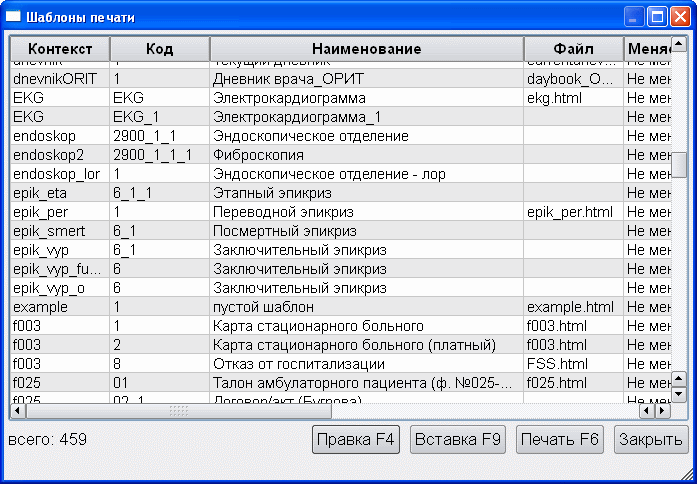
\includegraphics[width = 0.7\textwidth ,keepaspectratio]{patt_list}
 \caption{Список шаблонов печатных форм}
 \label{img_patt_list}
\end{figure}

\begin{figure}[ht]\centering
 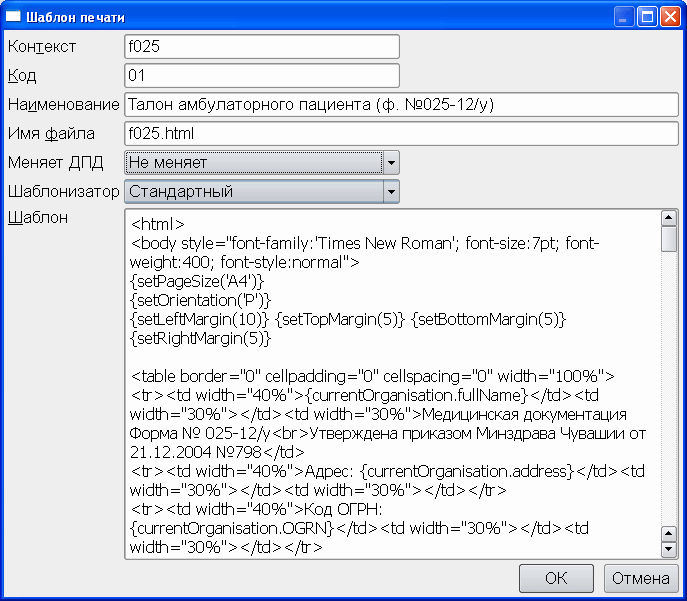
\includegraphics[width = 0.7\textwidth ,keepaspectratio]{patt_card}
 \caption{Карточка редактирования шаблона печати}
 \label{img_patt_card}
\end{figure}

Для регистрации нового шаблона печатной формы нужно нажать кнопку \btn{Вставка F9}. В открывшемся окне (Рисунок \ref{img_patt_card}) следует указать следующие параметры:
\begin{itemize}
 \item \dm{Контекст} – наименование контекста печати. С помощью данного поля происходит определение места вызова печатной формы. Как правило, печатные формы вызываются из карточки редактирования события (вкладка \dm{Основная информация}) или действия при нажатии кнопки \btn{Печать}. Для того чтобы шаблон печати вызывался из карточки редактирования определенного типа события (или действия) необходимо, чтобы значение данного поля совпадало со значением поля \dm{Контекст печати} справочника \dm{Типы событий} (\dm{Типы действий}). Рекомендуется в качестве значений поля \dm{Контекст} использовать короткие сочетания цифр, английских букв, знаков тире и подчеркивание. Существуют так же предопределенные значения контекста. Например, при указании значения <<token>>, шаблон печати будет вызываться из окна картотеки пациентов.
 \item \dm{Код} – для каждого контекста печати может быть задано несколько шаблонов печатных форм. Значение данного поля задает последовательность расположения шаблонов печати в контекстном меню кнопки \btn{Печатать} заданного окна.
 \item \dm{Наименование} – название печатной формы, отображаемое в контекстном меню кнопки \btn{Печатать}.
 \item \dm{Имя файла} – название файла шаблона печатной формы, если он хранится на рабочей станции.
 \item \dm{Меняет ДПД} – задает изменение значения идентификатора ДПД при вызове печати данного шаблона. Так, для печатных форм типа <<Информированное согласие …>> рекомендуется устанавливать значение данного поля в <<Меняет на <<Да>>. Тогда после печати формы на основе данного шаблона, в карточке пациента будет сделана отметка о получении от него согласия на проведение лечения.
 \item \dm{Шаблонизатор} – выбор типа шаблонизатора из списка. В зависимости от выбранного типа, нужно использовать различный синтаксис при создании шаблона печатной формы.
 \item \dm{Шаблон} – скрипт шаблона печатной формы, сохраняемый в БД.
\end{itemize}

\subsection{Структура шаблонов печатных форм}

Любой шаблон печатной формы представляет собой html-скрипт, содержащий специальные переменные и выражения. Переменные и выражения оформляются в соответствии с синтаксисом выбранного типа шаблонизатора.

На текущий момент ФТМИС поддерживается 2 типа шаблонизаторов, синтаксис которых различен:
\begin{enumerate}
 \item Стандартный;
 \item Jinja2.
\end{enumerate}
 
При настройке новых шаблонов печатных форм рекомендуется использовать шаблонизатор jinja2, т.к. он предоставляет более широкие возможности по созданию шаблонов.

\subsubsection{Синтаксис стандартного шаблонизатора}

При использовании стандартного шаблонизатора все операторы и выражения обрамляются в фигурные скобки. Например, \code{\{setPageSize ('A4')\}} или \code{\{for: prop in action\}}.

В общем случае, операторы могут иметь следующий формат:
\code{\{<ключевое слово>:<выражение>\}} или \code{\{<выражение>\}}.

В качестве ключевых слов могут быть использованы: \code{if}, \code{elif}, \code{else}, \code{for}, \code{end}.

При использовании первого варианта выражения (с ключевым словом), значение выражения определяется ключевым словом.

При использовании второго варианта выражения (без ключевого слова), оно, как правило, выполняет роль оператора вывода на печать. Например, \code{\{client.fullName\}} – вывод на печать ФИО пациента. Исключением является установка опций печати, например, \code{\{setPageSize('A4')\}}.

Если в выражении используются строки, то необходимо использовать префикс <<u>> (unicode), например \code{\{if: action.name == u"Поступление"\}\{: currentAction = action\}\{end:\}}.

Опции, задающие формат листа для печати:
\begin{itemize}
 \item \verb|{setPageSize('A4')}| – размер листа для печати;
 \item \verb|{setOrientation('P')}| – ориентация листа при печати: <<P>> – книжная, <<L>> – альбомная;
 \item \verb|{setMargins(10)}| – задает поля листа (одинаковое поле со всех сторон);
 \item \verb|{setLeftMargin(15)}| – задает левое поле;
 \item \verb|{setRightMargin(15)}| – задает правое поле;
 \item \verb|{setTopMargin(15)}| – задает верхнее поле;
 \item \verb|{setBottomMargin(15)}| – задает нижнее поле.
\end{itemize}

\paragraph{Оператор условия}

Общий вид оператора условия: 
\begin{verbatim}
{if: <условие>} 
<действие1> [<действие2>] … [<действиеN]
<!--Выполняются при выполнении условия --> 
[{elif: <условие2 (проверяется, если не выполнилось основное условие>} 
<действие2_1> [<действие2_2>] … [<действие2_N]] 		
<!-- Выполняются, если основное условие не выполняется, а условие2 выполняется  --> 
[{else:} 
<действие3_1> [<действие3_2>] … [<действие3_N]] 	
<!—Выполняются, если основное условие и условие2 не выполнены --> 
{end:} 
\end{verbatim}

При задании условия могут использоваться операторы сравнения: == (равно), != (не равно), <, >, <=, >=. Могут быть использованы сложные условия, объединенные с помощью ключевых слов \code{AND}, \code{OR}, \code{NOT}. \\

\opr{Пример1:} ~Для первой позиции в списке печатается значение <<Первая позиция>>, для остальных – <<Последующая позиция>>.
\begin{verbatim}
{if: k==0}{:k=1} 
<hr>Первая позиция <br>
{else:}
{:k=k+1}
Последующая позиция <br>
{end:}
\end{verbatim}

\opr{Пример2:} ~Если наименование текущего действия<<Поступление>>, то ссылка на него сохраняется в переменной \code{currentAction}.
\begin{verbatim}
{if: action.name == u"Поступление"}{: currentAction = action}{end:}
\end{verbatim}

Существует еще один вариант организации условия в стандартном шаблонизаторе. Принцип его работы аналогичен функции \code{iif} во многих языках программирования. В общем виде он выглядит следующим образом:

\verb|{<действие1> if <условие> else <действие2>}|

Описанная функция может использоваться как в качестве действия, так и в качестве части действия. Например: \begin{verbatim}
{: string = u"д. " + client.regAddress.number +
 ((u" корп. " + client.regAddress.corpus) 
 if (client.regAddress.corpus != "") else "") + u" кв. " +
  client.regAddress.flat}.
\end{verbatim} 
В описанном примере функция условия (помещена в круглые скобки) добавляет в адресную строку информацию о корпусе, только если это поле заполнено.

\paragraph{Оператор цикла} 

Общий вид оператора цикла:
\begin{verbatim}
{for: <переменная цикла> in <область значений переменной>}
<действие1>
[<действие2>]
…
[<действиеN>]
{end:}
\end{verbatim}

\opr{Пример3}: ~Поиск действия <<Поступление>> среди действий события.
\begin{verbatim}
{for: action in event.actions}
{if: action.name == u"Поступление"}{: currentAction = action}{end:}
{end:}
\end{verbatim}

\subsubsection{Организация диалогов}

При создании отчетов можно организовать получение входных значений посредством организации диалогов с пользователем. Для отображения диалогового окна следует использовать объект \code{dialogs}. В зависимости от выбранного метода, в результате работы диалога будет получено значение переменной определенного типа. Например, \code{\{: StrKod = dialogs.dialString(u"Введите код МКБ заболевания").getVar()\}} позволяет получить значение кода МКБ заболевания в виде строки. Можно использовать следующие методы объекта \code{dialogs}:
\begin{itemize}
 \item \code{dialBool} – диалог ввода логического значения;
 \item \code{dialDate} – диалог ввода даты;
 \item \code{dialFloat} – диалог ввода числа с плавающей точкой;
 \item \code{dialInt} – диалог ввода целого числа;
 \item \code{dialList} – диалог выбора значения из списка;
 \item \code{dialMultiList} – диалог выбора множественных значений из списка;
 \item \code{dialString} – диалог ввода строки;
 \item \code{dialTime} – диалог ввода времени.
\end{itemize}
 
Для всех перечисленных типов диалогов в качестве первого параметра указывается название диалога. Для методов \code{dialList} и \code{dialMultiList} указывается так же второй параметр – список значений в квадратных скобках. Для получения выбранного значения следует использовать метод \code{getVar()}.

\subsubsection{Функции работы с датами}

Функции определения текущей даты и времени:
\begin{itemize}
 \item \verb|{currentDate}| – текущая дата;
 \item \verb|{currentTime}| – текущее время.
\end{itemize}
 
Для задания формата вывода даты и времени используются методы \\ \code{date.toString(<формат>)} и \code{time.toString(<формат>)}. Например, \\ \code{action.endDate.date.toString('dd.MM.yyyy')} или  \code{action.begDate.time. toString('hh:mm')}.

Метод \code{daysTo(<конечная дата>)} возвращает количество дней от указанной даты до конечной. Например, \code{event.setDate.date.daysTo(currentDate. date)}.

Метод \code{addDays(<количество>)} увеличивает (либо уменьшает при указании отрицательного числа) дату на указанное количество дней. Например, \code{\{: currDate = act.begDate.date.addDays(1)\}} показывает день, следующий за \code{begDate}.

\subsection{Синтаксис шаблонизатора Jinja2}

В качестве альтернативы стандартному шаблонизатору в ФТМИС был добавлен шаблонизатор jinja2. В отличии от стандартного шаблонизатора, который является частью ФТМИС, jinja2 разрабатывается и поддерживается командой сторонних разработчиков. Это достаточно крупный проект с открытым исходным кодом (open source). Jinja2 предоставляет более широкие возможности для разработки шаблонов. Конструкции языка соответствуют общепринятым стандартам, более четкие и выверенные по сравнению со стандартным шаблонизатором.

Синтаксис шаблонизатора jinja2 имеет общие черты с синтаксисом стандартного шаблонизатора, но имеет и заметные отличия.

В шаблонизаторе jinja2 операторы могут обрамляться в двойные фигурные скобки \verb|{{ … }}| или фигурные скобки и знаки процента \verb||. Например, \code{\{\{setPageSize('A4')\}\}} или \code{\{\%for: prop in action\%\}}. Обрамление \verb|| используется для исполняемых операторов. Обрамление \verb|{{ … }}|, выполняет роль оператора вывода на печать. В обрамлении \verb|{# … #}| записываются комментарии.

\begin{vnim}
 В отличии от стандартного шаблонизатора, в Jinja2 не нужно добавлять префикс <<u>> перед строками. Например,  \{\%if action.name == "Поступление"\%\} \{\% currentaction = action \%\} \{\% endif \%\}
\end{vnim}
 
В jinja2 существует 2 способа обращения к свойствам переменных:
\begin{enumerate}
 \item \verb|{{new_var.prop1}}|;
 \item \verb|{{new_var['prop1']}}|.
\end{enumerate}

Оба они позволяют получить значение свойства переменной, однако, во втором случае сначала будет осуществляться поиск записи \verb|'prop1'| в \verb|new_var|, а только затем поиск свойства \verb|prop1|. В первом случае поиск происходит в обратном порядке.

Опции, задающие формат листа для печати:
\begin{itemize}
 \item \verb|{{setPageSize('A4')}}| – размер листа для печати;
 \item \verb|{{setOrientation('P')}}| – ориентация листа при печати: «P» – книжная, «L» – альбомная;
 \item \verb|{{setMargins(10)}}| – задает поля листа (одинаковое поле со всех сторон);
 \item \verb|{{setLeftMargin(15)}}| – задает левое поле;
 \item \verb|{{setRightMargin(15)}}| – задает правое поле;
 \item \verb|{{setTopMargin(15)}}| – задает верхнее поле;
 \item \verb|{{setBottomMargin(15)}}| – задает нижнее поле.
\end{itemize}
 
\subsubsection{Оператор условия}

Общий вид оператора условия:
\begin{verbatim}

<действие1> [<действие2>] … [<действиеN]	{# Выполняются при 
выполнении условия #}
[
<действие2_1> [<действие2_2>] … [<действие2_N]]	{# Выполняются, если
 основное условие не выполняется, а условие2 выполняется #}
[
<действие3_1> [<действие3_2>] … [<действие3_N]]	{# Выполняются, если
 основное условие и условие2 не выполнены #}

\end{verbatim}

Следует обратить внимание, что в Jinja условный оператор всегда заканчивается ключевым словом \code{endif}, а не \code{end}, как в стандартном шаблонизаторе.

При задании условия могут использоваться операторы сравнения: == (равно), != (не равно), <, >, <=, >=. Могут быть использованы сложные условия, объединенные с помощью ключевых слов \code{AND}, \code{OR}, \code{NOT}.

\opr{Пример4:} ~Выводится значение k. Если оно отрицательное, то печатается жирным (без знака). Если оно равно нулю, то значение выводится текстом.
\begin{verbatim}

<li>{{k}}</li>

<li><b>{{-k}}</b></li>

<li>Ноль</li>

\end{verbatim}

\subsubsection{Оператор цикла}

Общий вид оператора цикла:
\begin{verbatim}

<действие1>
[<действие2>]
…
[<действиеN>]

\end{verbatim}

Как и в предыдущем пункте, цикл заканчивается специальным ключевым словом \code{endfor}.

\opr{Пример5:} ~Вывод на печать значений свойств.
\begin{verbatim}
 
<td align="left">{{prop[0]}}</td> 
<td align="center">{{prop[2]}}</td>

\end{verbatim}

\subsubsection{Организация диалогов}

При создании отчетов с параметрами можно организовать диалоги с пользователем. Для отображения диалогового окна следует использовать объект \code{dialogs}. В зависимости от выбранного метода, в результате работы диалога будет получено значение переменной определенного типа. Например, \verb|| позволяет получить значение переменной \code{DataVVn} типа дата. Список методов объекта \code{dialogs} приведен в таблице \ref{tbl_patt_jdlg}.

{\small
\begin{longtable}{|p{3cm}|p{4.7cm}|p{9cm}|}
\caption{Типы диалогов \label{tbl_patt_jdlg}} \\
\hline \rule{0pt}{15pt} \centering \textbf{Название} & \centering \textbf{Аргументы} & \hfil \textbf{Описание} \\ \hline
\endfirsthead
\hline \rule{0pt}{15pt} \centering \textbf{Название} & \centering \textbf{Аргументы} & \hfil \textbf{Описание} \\ \hline
\endhead
dialBool &	Название диалога	& Ввод значения переменной логического типа  \\ \hline
dialDate &	Название диалога &	Ввод значения переменной типа дата \\ \hline
dialInt	& Название диалога	& Ввод значения целочисленной переменной \\ \hline
dialFloat &	Название диалога &	Ввод значения переменной с плавающей точкой \\ \hline
dialMultiList &	Название диалога, список значений &	Выбор нескольких значений из списка. Список доступных значений заключается в квадратные скобки. Для получения значения функции, следует применять метод \code{getListValues()}. Например, \code{dialogs.dialMultiList("Выберите элемент (ы) из списка}\verb|",["1", "2", "3"]).| \code{getListValues()} \\ \hline
dialList	& Название диалога, список значений	& В отличии от предыдущего элемента, в данном случае можно выбрать только одно значение из предложенного списка \\ \hline
dialOrg	& Название диалога	& Выбор значения переменной из справочника организаций \\ \hline
dialOrgStructure	& Название диалога	& Выбор подразделения из организационной структуры ЛПУ \\ \hline
dialPerson	& Название диалога &	Выбор сотрудника из справочника сотрудников \\ \hline
dialRB	& Название диалога, название таблицы БД справочника	& Выбор значения переменной из справочника, название которого указано в качестве второго аргумента (название справочника указывается в двойных кавычках). В данном типе диалога могут быть использованы следующие методы: \begin{itemize}
 \item \code{getId()} – возвращает идентификатор выбранной записи;
 \item \code{getCode()} – возвращает код выбранной записи (из поля Code справочника);
 \item \code{getName()} – возвращает название элемент справочника;
 \item \code{getVar()} – возвращает значение элемента справочника (поле \code{Code} либо его аналог), может использоваться для справочников, не имеющих поля \code{Code}.
\end{itemize}  
Например, \code{dialogs.dialRB("Выберите вид полиса"}\verb|, "rbPolicyType").getCode()| \\ \hline
dialService	& Название диалога	& Выбор услуги из справочника \mm{Услуга (профиль ЕИС)}. Могут быть использованы методы \code{getId()}, \code{getCode()}, \code{getName()}, описанные в предыдущем пункте \\ \hline
dialString	& Название диалога	& Ввод значения переменной символьного типа (строки) \\ \hline
dialTime	& Название диалога &	Ввод значения переменной типа время \\ \hline
\end{longtable}
}

Для получения значения в типах диалогов, для которых в таблице \ref{tbl_patt_jdlg} не указаны доступные методы, следует использовать метод \code{getVar()}.

\subsubsection{Использование фильтров}

Фильтрами в jinja называются функции преобразования (изменения) переменных. Например, преобразования типов, обработки строк, форматирования, математические функции и др.

В общем виде применение фильтра выглядит следующим образом:
\begin{verbatim}
<результирующая переменная> = <исходная
переменная>|функция[(<аргумент2>[,<аргумент3>…[,<аргументN>]])]
\end{verbatim}

Т.е. в начале указывается переменная, к которой следует применить фильтр (функцию), затем ставится вертикальная черта и указывается название фильтра. В скобках после названия фильтра могут указываться дополнительные аргументы (основным аргументом является переменная). Например, \code{summa = 0|float}.

Можно последовательно применить к переменной несколько фильтров. Например, в результате записи \verb/{{ 42.55|round|int }}/ будет получено значение 43. Сначала будет произведено округление числа 42.55 до 0 знаков после запятой (=43.0), а затем преобразование полученного результата к целому (= 43).

Наиболее часто используемые фильтры:
\begin{itemize}
 \item \code{<число>|abs} – возвращает абсолютное значение числа.
 \item \code{<переменная>|center(<ширина>)} – выравнивает по центру значение указанной переменной в поле заданной ширины (по умолчанию = 80).
 \item \code{<переменная>dictsort(<чувствительность к регистру>,<поле сортировки>)} – сортирует переменную типа словарь, образуя на выходе пары (ключ, значение). В качестве дополнительных параметров сортировки можно задать чувствительность к регистру = \code{True} (по умолчанию – \code{False}) и поле для сортировки: \code{‘key’} – по ключу (по умолчанию), \code{‘value’} – по значению.
 \item \code{<строка>|escape} – преобразует символы \verb|&, <, >, ‘, ”| в html-теги.
 \item \code{<последовательность>|first} – возвращает первый элемент последовательности;
 \item \code{<переменная>|float(<значение по умолчанию>)} – преобразование переменной к формату числа с плавающей точкой. В случае ошибки преобразования, функция возвращает значение по умолчанию (по умолчанию оно равно 0.0);
 \item \code{<последовательность>|groupby(<атриббут>)} – выполняет группировку последовательности по заданному атрибуту;
 \item \code{<строка>|indent(<отступ>,<делать отступ для первой строки>)} – добавляет отступы на указанное в параметре «отступ» число пробелов (по умолчанию – 4). Для первой строки по умолчанию отступ не делается. Для того чтобы отступ был добавлен и в первую строку, необходимо установить значение параметра «делать отступ для первой строки» в \code{True};
 \item \code{<переменная>|int(<значение по умолчанию>)} – преобразует переменную к целочисленному типу. Если преобразование не удалось, функция возвращает значение по умолчанию (по умолчанию – 0).
 \item \code{<последовательность>|last} – возвращает последний элемент последовательности;
 \item \code{<последовательность>|length} – возвращает длину (количество элементов) последовательности. Можно так же использовать функцию \code{count};
 \item \code{<строка>|lower} – преобразование строки к нижнему регистру;
 \item \code{<переменная>|round(<точность>,<метод>)} – округляет переменную. В параметре «точность» следует указать количество знаков после запятой, до которого следует производить округление (по умолчанию – 0). Параметр \code{метод} указывает способ округления: \code{common} - округление производится по правилам математики, \code{ceil} - всегда округляется в большую сторону, \code{floor} - всегда округляется в меньшую сторону (по умолчанию – \code{common}).
 \item \code{<строка>|striptags} – вычищает html-теги и удаляет двойные пробелы;
 \item \code{<строка>|title} – возвращает строку, где первая буква в верхнем регистре, а остальные – в нижнем;
 \item \code{<строка>|trim} – удаляет пробелы в начале и в конце строки;
 \item \code{<строка>|truncate(<длина>,<по словам>,<символ завершения>)} – обрезает строку до указанного количества символов в поле \code{длина} (по умолчанию – 255). Если параметр \code{по словам = False} (по умолчанию), то при попадании границы обрезки на середину слова, неполная часть его будет отброшена; при установке параметра в \code{True} часть слова будет включена в результат. Например, \verb/{{ "foo bar"|truncate(5) }} => "foo ..."/, но \verb/{{ "foo bar"|truncate(5, True) }} => "foo b..."/. Параметр \code{символ завершения} указывает, каким символом (символами) будет закончена строка (по умолчанию – <<…>>).
 \item \code{<строка>|upper} – преобразует строку к верхнему регистру.
\end{itemize}
 
Это далеко не полный перечень доступных фильтров. Полный список фильтров можно найти на сайте разработчиков jinja2 в разделе технической документации http://jinja.pocoo.org/docs/.

\subsubsection{Функции работы с датами}

Для задания формата вывода даты и времени на печать необходимо использовать функции \verb| date_toString(<переменная>,<формат>)| и \verb|time_toString(<переменная>,<формат>)| соответственно. Например, \verb|{{date_toString(action.begDate.date, 'dd.MM.yyyy')}}| или \verb|time_toString(action.begDate.time, 'hh.mm')|.

\subsubsection{Особенности работы с переменными в цикле}

В шаблонизаторе jinja2 для повышения производительности используется <<правильная>> область видимости переменных. В связи с этим могут возникать ситуации, когда переменная, значение которой установлено в логическом блоке (например, цикле) принимает свое исходное значение вне него.

Например, при попытке получения диагноза последнего осмотра с помощью следующего кода, будет получено пустое значение:
\begin{verbatim}

   
      
       
         
            
         
      
   

\end{verbatim}

Как уже говорилось выше, в результате выполнения данного кода переменная \code{diag} обнуляется при выходе из цикла. Для того чтобы избежать данного эффекта, рекомендуется использовать массивы. Их область видимости глобальна. Тогда приведенный выше пример, нужно изменить следующим образом:
\begin{verbatim}


   
      
       
         
            
         
      
   

\end{verbatim}

\subsection{Контексты печати} \index{Листы назначений (настройки)}

\opr{Контекст печати} – это совокупность передаваемых шаблонизатору объектов, которые могут им использоваться при отображении шаблона.

Контексты печати определяются местом, откуда производится печать. Например:
\begin{itemize}
 \item При вызове шаблона с вкладки \dm{Основная информация} какого-либо события используется контекст печати \code{event}. При этом доступна информация о событии, всех действиях этого события и их свойствах. Подробное описание контекста \code{event} приведено в таблице  \ref{tbl_patt_prn_ev}.
 \item При вызове печати из карточки редактирования действия, используется контекст печати \code{action}. При этом доступна информация о текущем действии и его свойствах, а так же о родительском событии. Подробное описание контекста \code{action} приведено в таблице \ref{tbl_patt_prn_act}.
 \item При вызове печати из карточки пациента, используется контекст \code{client} типа \code{CClienInfo}. При этом становится доступной для вывода на печать персональная информация о пациенте.
\end{itemize}
 
Выше перечислены основные места вызова печати, но существуют так же специальные места вызова. Для них могут создаваться собственные контексты печати. Например, для отображения общей информации о пациенте в верхней части окна картотеки пациентов используется контекст \verb|__client_info| типа \code{CClienInfoFrame}, содержащий данные о пациенте, выбранном событии и некоторые дополнительные данные. Для него существует 2 кода: \verb|__normal| для отображения данных о выбранном пациенте и \verb|__empty| если пациент не выбран.

Для печати листов назначений необходимо использовать контекст печати \verb|__prescription|. Для печати листа исполнений – контекст \verb|__prescription_all|. Для печати шапки листа назначений следует использовать контекст печати \verb|__client_info| и название шаблона <<\_\_prescriptions>>.

{\small
\begin{longtable}{|p{4cm}|p{5cm}|p{7.6cm}|}
\caption{Описание контекста event \label{tbl_patt_prn_ev}} \\
\hline \rule{0pt}{15pt} \centering \textbf{Наименование объекта} & \centering \textbf{Тип} & \hfil \textbf{Описание} \\ \hline
\endfirsthead
\hline \rule{0pt}{15pt} \centering \textbf{Наименование объекта} & \centering \textbf{Тип} & \hfil \textbf{Описание} \\ \hline
\endhead
eventType &	CEventTypeInfo	& Тип обращения \\ \hline
externalId	& Unicode	& Внешний идентификатор \\ \hline
setDate	& CDateTimeInfo	& Дата назначения \\ \hline
execDate	& CDateTimeInfo	& Дата выполнения \\ \hline
org	& COrganisationInfo	& Организация \\ \hline
client	& CClientInfo	& Пациент \\ \hline
contract	& CContractInfo	& Договор \\ \hline
prevEventDate	& CDateTimeInfo	& Дата предыдущего обращения \\ \hline
setPerson	& CPersonInfo	& Кем направлен \\ \hline
execPerson	& CPersonInfo	& Выполнил \\ \hline
isPrimary	& bool	& Признак первичности обращения \\ \hline
order	& int	& Порядок поступления (код) \\ \hline
result	& CResultInfo	& Результат обращения \\ \hline
acheResult	& CAcheResultInfo &  \\ \hline 	
nextEventDate	& CDateTimeInfo	& Дата следующего обращения \\ \hline
payStatus	& int	& Источник финансирования (код) события \\ \hline
typeAsset	& CEmergencyTypeAssetInfo &  \\ \hline	
note	& Unicode	& Примечание \\ \hline
curator	& CPersonInfo	& Куратор \\ \hline
assistent &	CPersonInfo	& Ассистент \\ \hline
actions	& CActionInfoList &	Действия, выполненные в рамках текущего события \\ \hline
diagnosises	& CDiagnosticInfoList &	Диагнозы, установленные в рамках текущего события \\ \hline
visits	& CVisitInfoList	& Посещения, выполненные в рамках текущего обращения \\ \hline
localContract	& CEventLocalContractInfo &  \\ \hline	
mes	& CMesInfo	& МЭС, связанный с данным обращением \\ \hline
mesSpecification &	CMesSpecificationInfo &	Особенности выполнения МЭС \\ \hline
\end{longtable}
}

{\small
\begin{longtable}{|p{4.1cm}|p{5cm}|p{7.5cm}|}
\caption{Описание контекста action \label{tbl_patt_prn_act}} \\
\hline \rule{0pt}{15pt} \centering \textbf{Наименование объекта} & \centering \textbf{Тип} & \hfil \textbf{Описание} \\ \hline
\endfirsthead
\hline \rule{0pt}{15pt} \centering \textbf{Наименование объекта} & \centering \textbf{Тип} & \hfil \textbf{Описание} \\ \hline
\endhead
event &	CEventInfo	& Ссылка на событие, в составе которого находится действие. Описание типа объекта CEventInfo приведено в таблице \ref{tbl_patt_prn_ev} \\ \hline
directionDate	& CDateTimeInfo	& Дата (и время) направления \\ \hline
begDate	& CDateTimeInfo	& Дата (и время) начала действия \\ \hline
plannedEndDate	& CDateTimeInfo	& Плановая дата (и время) выполнения \\ \hline
endDate	& CDateTimeInfo &	Дата (и время) выполнения \\ \hline
isUrgent & 	bool	& \\ \hline
coordDate	& CDateTimeInfo & \\ \hline	
coordAgent	& Unicode	&  \\ \hline
coordInspector	& Unicode & \\ \hline	
coordText	& Unicode	&  \\ \hline
status	& int	& Состояние действия (код) \\ \hline
office	& Unicode	& Кабинет \\ \hline
note	& Unicode	& Примечание \\ \hline
amount	& double	& Количество \\ \hline
setPerson	& CPersonInfo	& Назначил \\ \hline
person	& CPersonInfo	& Исполнитель \\ \hline
expose	& bool &  \\ \hline	
account	& bool &  \\ \hline	
price	& double &	Стоимость \\ \hline
finance	& CFinanceInfo	& Источник финансирования (код) \\ \hline
action\_id	& int	& Идентификатор записи \\ \hline
takenTissueJournal\_id	& int	& Идентификатор записи в журнале работ \\ \hline
takenTissue	& CTakenTissueJournalInfo	&  \\ \hline
\end{longtable}
}

{\small
\begin{longtable}{|p{4.1cm}|p{5cm}|p{7.5cm}|}
\caption{Описание контекста client\_info \label{tbl_patt_prn_cl}} \\
\hline \rule{0pt}{15pt} \centering \textbf{Наименование объекта} & \centering \textbf{Тип} & \hfil \textbf{Описание} \\ \hline
\endfirsthead
\hline \rule{0pt}{15pt} \centering \textbf{Наименование объекта} & \centering \textbf{Тип} & \hfil \textbf{Описание} \\ \hline
\endhead
client	& CClientInfo	& Ссылка на описание выбранного пациента \\ \hline
event &	CEventInfo	& Ссылка на описание события (если оно выбрано) \\ \hline
bedLabel	& Unicode &	Название койки размещения пациента \\ \hline
deptLabel	& Unicode &	Название отделения госпитализации пациента \\ \hline
disability	& Unicode &	Инвалидность \\ \hline
agreeText	& Unicode &	Согласие \\ \hline
showDocs	& bool	& Признак <<Показывать документы>> \\ \hline
\end{longtable}
}

\subsection{Специальные переменные} \label{patt_svar}

\opr{Специальная переменная} – это переменная, значением которой является результат SQL-запроса.

Чтобы использовать специальную переменную в тексте шаблона необходимо предварительно добавить ее в список специальных переменных в пункте меню \mm{Настройка \str Настройка специальных переменных} (Рисунок \ref{img_patt_svar}).

\begin{figure}[ht]\centering
 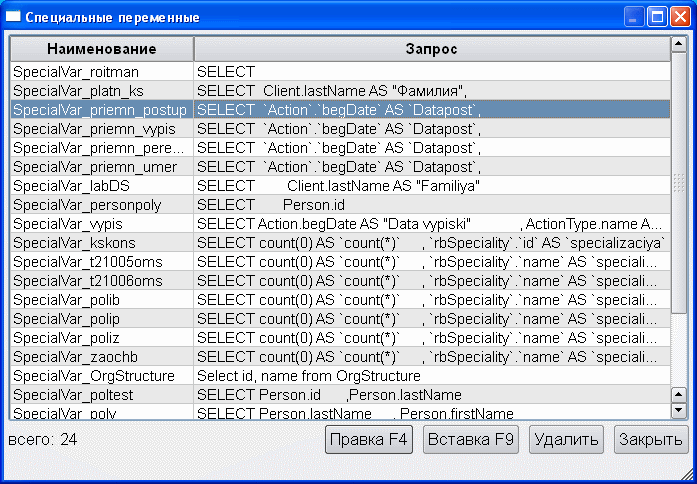
\includegraphics[width = 0.8\textwidth ,keepaspectratio]{patt_svar}
 \caption{Список специальных переменных}
 \label{img_patt_svar}
\end{figure}

\begin{figure}[ht]\centering
 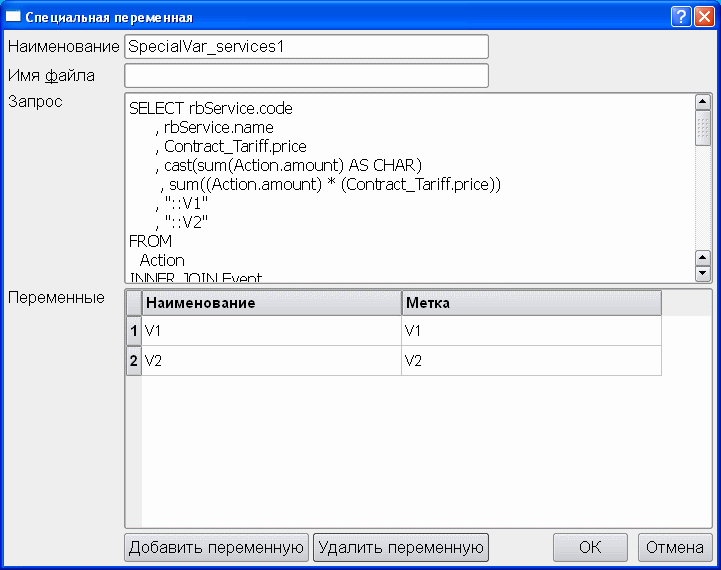
\includegraphics[width = 0.8\textwidth ,keepaspectratio]{patt_svar_card}
 \caption{Окно редактирования специальной переменной}
 \label{img_patt_svar_card}
\end{figure}

При добавлении новой специальной переменной необходимо указать (Рисунок \ref{img_patt_svar_card}):
\begin{itemize}
 \item \dm{Наименование переменной}. Оно должно быть уникально в списке специальных переменных и начинаться с префикса <<\code{SpecialVar\_}>>.
 \item \dm{Имя файла} – имя файла, содержащего SQL-запрос. Файл должен иметь расширение *.txt и располагаться в папке <<sqlqueries>> клиентского приложения.
 \item \dm{Запрос} – если имя файла в предыдущем поле не указано, то можно ввести текст SQL-запроса непосредственно в данное поле.
 \item \dm{Переменные}. Необходимо добавить в таблицу все переменные (параметры), участвующие в SQL-запросе, используя кнопки \btn{Добавить переменную} и  \btn{Удалить переменную}.
\end{itemize}

Текст SQL-запроса должен быть записан в след виде:

\verb|SELECT * FROM tablename where fio=::v1 and date=::v2;|

где \code{v1,v2} - переменные для SQL-запроса, значения которых указываются в тексте шаблона или вводятся с клавиатуры через механизм организации диалогов.

Для задания значений переменных, которые будут использоваться в SQL-запросе, в тексте шаблона необходимо использовать функцию \code{SpecialVariable()}. Первым аргументом функции нужно указать наименование переменной, а последующие переменные должны содержать значения всех переменных для SQL-запроса в том порядке, в котором они были описаны при создании специальной переменной.

Например, имеется специальная переменная \verb|SpecialVar_name1|, для которой заданы переменные \code{id} и \code{name}. Необходимо передать значение \code{id} равным 3 и значение \code{name} равным <<Name1>>. Для этого необходимо использовать конструкцию:

\verb|SpecialVariable('SpecialVar_name1', 3,'Name1')|

Для вывода на печать значения специальной переменной используется конструкция:
\begin{verbatim}

   
   {{i}}
   

\end{verbatim}

\subsection{Создание аналитических отчетов}

Для создания аналитического отчета необходимо:
\begin{itemize}
 \item Создать соответствующий шаблон печати в меню \mm{Настройки \str Шаблоны печати} (см. п. \ref{patt_add}). Как правило, при создании шаблонов печати для аналитических отчетов используются специальные переменные (см. п. \ref{patt_svar})
 \item Добавить аналитический отчет в меню  \dm{Настройки  \str Настройка свободных отчетов} (Рисунок \ref{img_patt_arep}). Добавление новых отчетов производится непосредственно в таблицу. Для этого нужно дважды щелкнуть левой кнопкой мыши в нижней (пустой) строке таблицы, активировав возможность ввода данных. В поле \dm{Наименование} нужно ввести с клавиатуры название отчета, как оно будет отображаться в меню, в поле \dm{Шаблоны печати} – выбрать из списка созданный на предыдущем шаге шаблон.
\end{itemize} 

\begin{figure}[ht]\centering
 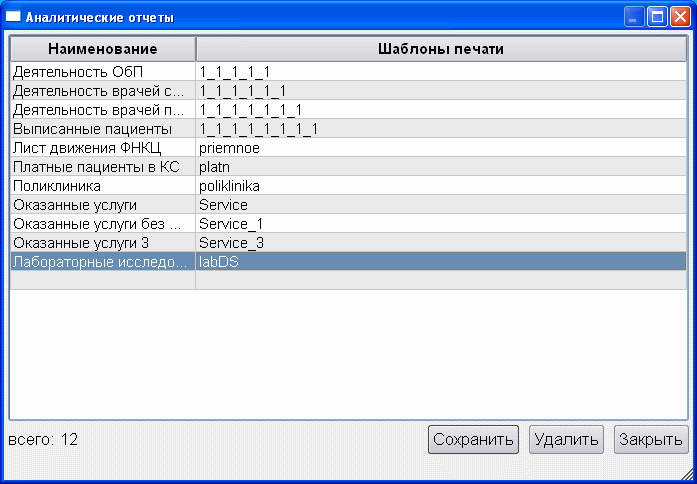
\includegraphics[width = 0.7\textwidth ,keepaspectratio]{patt_arep}
 \caption{Окно добавления аналитических отчетов}
 \label{img_patt_arep}
\end{figure}

После выполнения указанных действий в пункте меню \mm{Анализ \str Аналитические отчеты} появится отчет с указанным наименованием.